\documentclass[11pt,twoside]{article}

\usepackage{blindtext}
\usepackage[T1]{fontenc}
\usepackage{microtype}
\usepackage[english]{babel}
\usepackage[hmarginratio=1:1,top=20mm,bottom=20mm,columnsep=20pt,left=30mm]{geometry}
\usepackage[hang, small,labelfont=bf,up,textfont=it,up]{caption}
\usepackage[page]{appendix}
\usepackage{float,graphicx,wrapfig,subcaption,booktabs,lettrine,enumitem,amsmath,}
\setlist[itemize]{noitemsep}
\usepackage{graphicx}

\usepackage{comment}


\usepackage{abstract}
\renewcommand{\abstractnamefont}{\normalfont\bfseries}
\renewcommand{\abstracttextfont}{\normalfont\small}

\usepackage{titlesec}
\titleformat{\section}[block]{\large\scshape\centering}{\thesection.}{1em}{}
\titleformat{\subsection}[block]{\large}{\thesubsection.}{1em}{}
\usepackage{titling}
\usepackage{hyperref}

%----------------------------------------------------------------------------------------
%   TITLE SECTION
%----------------------------------------------------------------------------------------

\setlength{\droptitle}{-4\baselineskip} % Move the title up

\pretitle{\begin{center}\Huge\bfseries} % Article title formatting
\posttitle{\end{center}} % Article title closing formatting
\title{Machine Learning} % Article title
\author{%
\textsc{Gianmarco Ricciarelli} \\[1ex] % Your name
\normalsize \href{mailto:john@smith.com}{gianmarcoricciarelli@gmail.com} % Your email address
\and % Uncomment if 2 authors are required, duplicate these 4 lines if more
\textsc{Stefano Carpita} \\[1ex] % Second author's name
\normalsize \href{mailto:jane@smith.com}{carpitastefano@gmail.com} % Second author's email address
}
\date{
    ML - Academic Year: 2018/2019 \\
    {\vspace{0.25cm}}
    \today \\
    {\vspace{0.25cm}}
    Type of project: \textbf{A} \\
    {\vspace{0.25cm}}
    \href{https://github.com/germz01/machinel-learning}{Github Page}
}
\renewcommand{\maketitlehookd}{%
\begin{abstract}
\noindent With this report we describe our type \textbf{A} project for the Machine Learning course. We experiment
two datasets, namely MONK's and CUP, by building from scratch a neural network's implementation, which we've
validated by searching for the best hyper-parameters' combination via well-known validation techniques. Finally,
for each one of the datasets, we collected the data describing the results.
\end{abstract}
}

\graphicspath{{img/}}
\setlength\parindent{0pt}

%----------------------------------------------------------------------------------------

\begin{document}

% Print the title
\maketitle

%----------------------------------------------------------------------------------------
%   ARTICLE CONTENTS
%----------------------------------------------------------------------------------------

\section{Introduction} % (fold)
\label{sec:introduction}
    By chosing a type \textbf{A} project, we followed the goal of building and optimizing a
    \textit{feedforward neural network model} by searching the best hyper-parameters' combination in order to
    obtain the best performances on the MONK's and CUP datasets. The model we've built implements the
    standard \textit{backpropagation algorithm} with \textit{gradient descent}, as described in
    \cite{deep_learning}. As optimization tool, we've searched the so-called hyper-parameters space by using
    well-known validation algorithms like \textit{k-fold cross validation} and \textit{(random) grid search},
    described in \cite{deep_learning} and \cite{random_search}. More technical details regarding the
    implementation can be found in section \ref{sec:methods}.
% section introduction (end)

%------------------------------------------------

\section{Methods} % (fold)
\label{sec:methods}
    Our code base is written using the \textit{Python} programming language, which was enhanced with
    numerical libraries like \textit{NumPy} and \textit{Pandas} to ease the computational cost involved in
    implementating popular machine learning algorithms. %%Also the standard library function provided by the language were utilized.
    Following the philosophy of type \textbf{A} projects, we haven't used
    out-of-the-box implementations for the algorithms composing our framework. We now give a brief overview of
    the code's structure, discuss some implementation choices and present our neural network's initialization
    and training algorithms. Visit the project's
    \href{https://github.com/germz01/machinel-learning}{\underline{\textit{Github Page}}} if you want to check
    our project's code base.

    \subsection{Code overview} % (fold)
    \label{sub:code_overview}
        We can view our code base essentialy divided in two branches: the \textit{neural network} branch and
        the \textit{model selection and assessment} branch. The first one is composed by the code for
        implementing the neural network model, and all the code related
        to the building and training of such a model, e.g. the activation functions, the losses, the
        regularization metrics and so on, that is divided in several scripts in order to ease the
        implementation. The code base's second branch consist in the model selection and assessment related
        code, which is composed by several classes, each one implementing an algorithm like \texttt{GridSearch}
        and \texttt{KFold\_Cross\_validation} which are utilized for the model's validation, selection and
        assessment, and the scripts that build up the testing routines for the MONK's and CUP datasets.
        The second branch also is splitted in several scripts.
    % subsection code_overview (end)

    \subsection{Implementation choices} % (fold)
    \label{sub:implementation_choices}
        Since we wanted to be able to take different paths during the building phase of our model, we enriched
        the first code base's branch by writing diffent activation functions, losses and regularization metrics.
        In the \texttt{activation} script we writed the code for the \texttt{sigmoid}, \texttt{relu},
        \texttt{tanh} and \texttt{identity} activation functions. The \texttt{regularizers} script contains the
        code for implementing both the $L^1$ and $L^2$ regularization metrics, as described in
        \cite{deep_learning}, and the \texttt{losses} script contains the code for implementing popular loss
        function like, for example, the \texttt{mean\_squared\_error} and the \texttt{mean\_euclidean\_error}.
        All this metrics are applied in the \texttt{nn} script, which contains the code for implementing the
        neural network model, and hence the backpropagation algorithm and the training algorithm, described in
        section \ref{sub:the_training_algorithm}. The \texttt{NeuralNetwork} class, which is contained in this
        script, represents a neural network using the standard \textit{backpropagation algorithm} with
        \textit{gradient descent}, \textit{standard momentum} and \textit{regularization}, and follows the
        \textit{minibatch} approach, as described in \cite{deep_learning}. The \texttt{NeuralNetwork} class
        contains also various early stopping metrics, like the $GL_{\epsilon}$ and the $PQ_{\epsilon}$ which we
        implemented following \cite{early_stopping}. More details about what particular combination of
        metrics was used during the experimental phase can be found in section \ref{sec:experiments}.

        \subsection{Network's initialization and training} % (fold)
        \label{sub:the_training_algorithm}
        Our neural network can be initialized for pursuing either a \textit{classification} task or a
        \textit{regression} one. The initialization phase for the two tasks is the same.
        During the initialization phase, we pass to the network the design matrix \texttt{X} and target column
        vector \texttt{y}. Other than that we pass the number of neurons per hidden layer
        \texttt{hidden\_sizes}, the maximum number of epochs \texttt{epochs}, the minibatch's size
        \texttt{batch\_size}, the activation function for each layer \texttt{activation} and the hyper-parameters
        for the learning rate, \texttt{$\eta$}, the momentum, \texttt{$\alpha$} and the regularization,
        \texttt{$\lambda$}. In order to initialize the network's weights matrices we followed the
        \textit{normalized initialization} technique, described in \cite{deep_learning} and
        \cite{initialization}, e.g. the formula defining the network's weights in the uniform distribution
        taken in the range

        \begin{equation*}
             W \sim U \left [ - \frac{\sqrt{6}}{\sqrt{m + n}}, \ \frac{\sqrt{6}}{\sqrt{m + n}}  \right ],
        \end{equation*}

        in which $m$ and $n$, respectively, represents the number of inputs and outputs for the layer.
        During the training phase we essentialy apply the \textit{forward propagation} and the
        \textit{backpropagation} phases of the standard \textit{backpropagation} algorithm over a minibatch of
        examples taken from the training set. During each epoch of training we also keep track of the errors
        between the predicted values and target ones, in order to be able to plot the \textit{learning curves}
        for the training session. At the end of each epoch the neural network's weights are updated following
        the standard backpropagation/momentum/regularization convention.
        % subsection the_training_algorithm (end)
    % subsection implementation_choices (end)
% section methods (end)

%------------------------------------------------

\section{Experiments} % (fold)
\label{sec:experiments}
    Before delving into the details of the results we obtained by applying our models to the MONKS and CUP
    datasets, we provide some informations about the \textit{preprocessing routines} and
    \textit{validation schema} we decided to apply. Since the MONKS datasets' feature are categorical, that is,
    every feature's value represents a class, not a numerical value, we preprocessed the three datasets by
    writing a \texttt{monks\_binarize} script for applying a \textit{1-of-k encoding}, as recommended during
    the course, hence obtaining $17$ binary input features. Since we've
    chosen to follow \cite{random_search} for the hyper-parameters' search during the validation phase, we first
    performed some \textit{preliminary trials} in order to have a glimpse on the best intervals for searching
    our model's hyper-parameters. During this trials we manually varied the model's hyper-parameters, e.g. the
    learning rate, the momentum constant and so on, and observed the resulting \textit{learning curves}
    (see appendix \ref{sec:preliminary_trials_learning_curves} for some examples).
    We then deepen the search using the most interesting intervals discovered during the preliminary trials
    in the validation phase by using our implementation of the \textit{(random) grid search} algorithm, in
    which we also used our implementation of the \textit{k-fold cross validation} algorithm (which follows
    the standard approach of using a value of $3$ for the \textit{k} parameter). That is, our validation schema
    essentially consist in using the random grid search algorithm to investigate some random sampled "points"
    in the hyper-parameters' space, evaluating the performances for each one of this points and finally
    selecting the best combinations of parameters based on the diffent metrics like \textit{generalization
    error}, \textit{accuracy}, \textit{precision} and \textit{f1-score}.

    \subsection{Monk's results} % (fold)
    \label{sub:monk_s_results}

    \begin{table}[H]
        \centering
        \begin{subtable}{\textwidth}
            \resizebox{\textwidth}{!}{
                \begin{tabular}{| c | c | c | c | c | c | c | c | c |}
                    \hline
                    Task & Topology & Batch size & Activation & $\eta$ & $\alpha$ & $\lambda$ & MSE (TR - TS) &
                    Accuracy (TR - TS) (\%) \\
                    \hline
                    MONK 1 & 17 -> 3 -> 1 & batch & sigmoid & 0.8 & 0.9 & 0.0 & 0.00223 - 0.00343 &
                    100 \% - 100 \% \\
                    \hline
                    MONK 2 & 17 -> 3 -> 1 & batch & sigmoid & 0.5 & 0.9 & 0.0 & 0.00125 - 0.00135 &
                    100 \% - 100 \% \\
                    \hline
                    MONK 3 & 17 -> 3 -> 1 & batch & sigmoid & 0.6 & 0.9 & 0.0 & 0.01668 - 0.03858 &
                    96.7 \% - 95.1 \% \\
                    \hline
                    MONK 3 (reg.) & 17 -> 3 -> 1 & batch & sigmoid & 0.6 & 0.9 & 0.01 & 0.05904 - 0.04669 &
                    93.4 \% - 97.2 \% \\
                    \hline
                \end{tabular}
            }
        \end{subtable}
        \caption{Average prediction results obtained for the MONK’s tasks.}
        \label{monks}
    \end{table}

    \begin{figure}[htbp]
        \centering
        \begin{subfigure}{0.90\textwidth}
            \resizebox{\textwidth}{!}{
                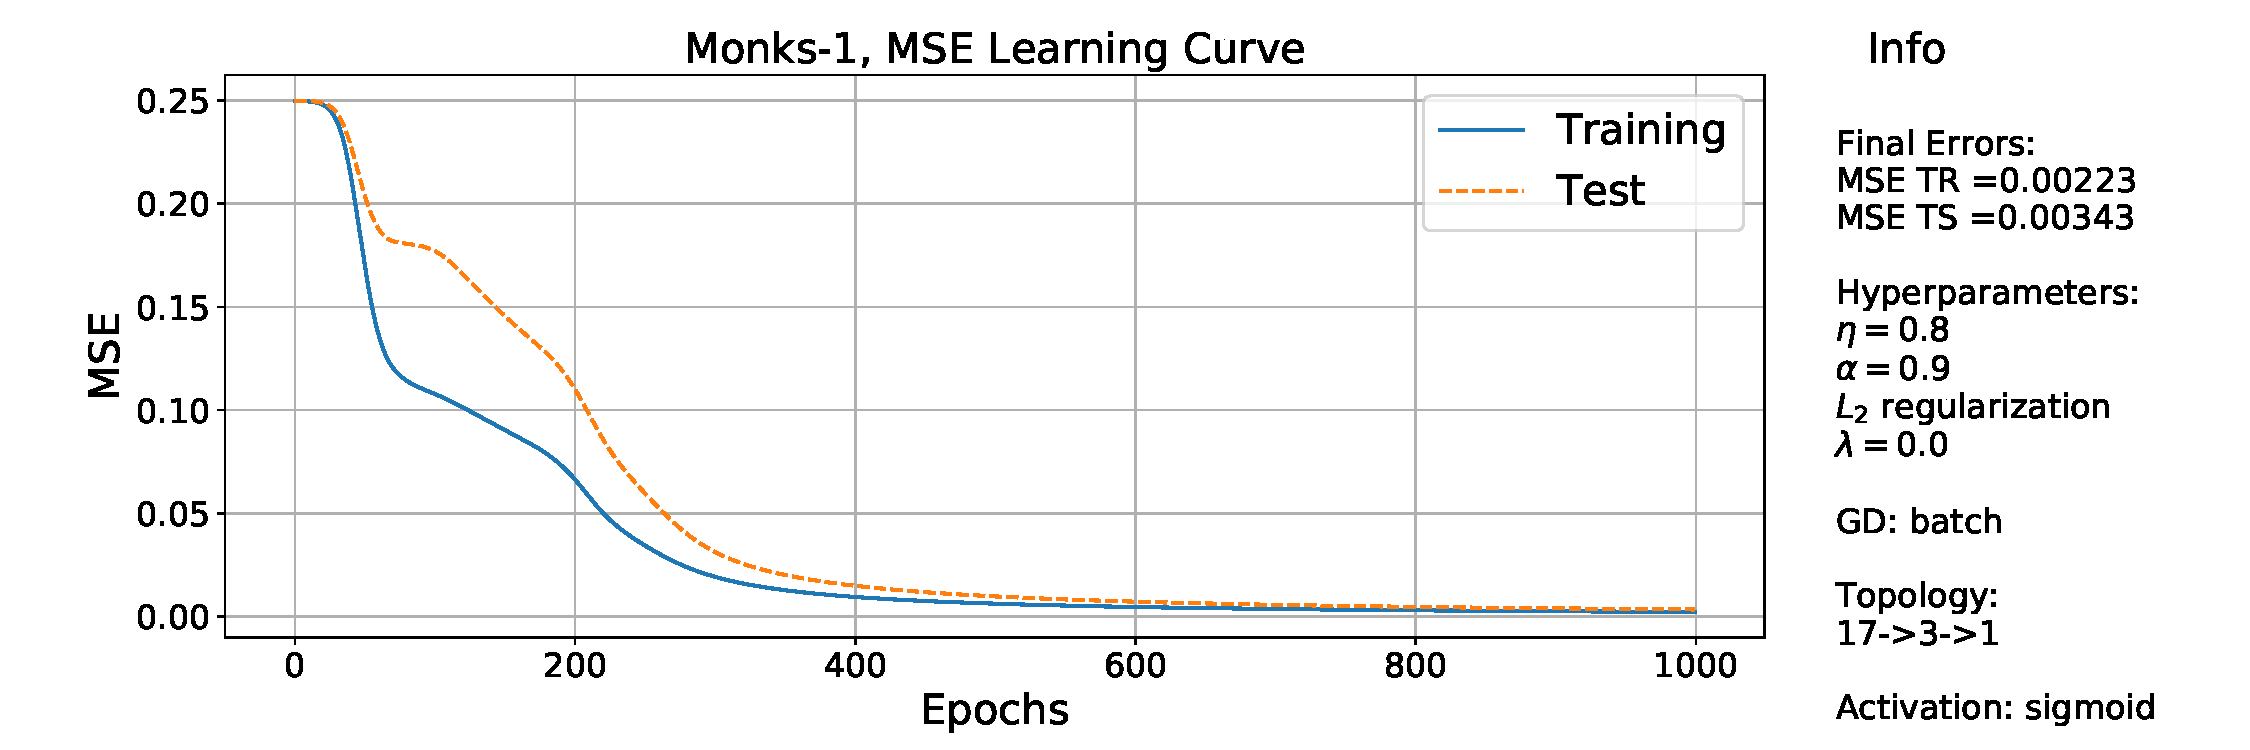
\includegraphics{img/monks_1_MSE_final_04.pdf}
            }
            \caption{}
            \label{fig:monks_1_MSE}
        \end{subfigure}
        \begin{subfigure}{0.90\textwidth}
            \resizebox{\textwidth}{!}{
                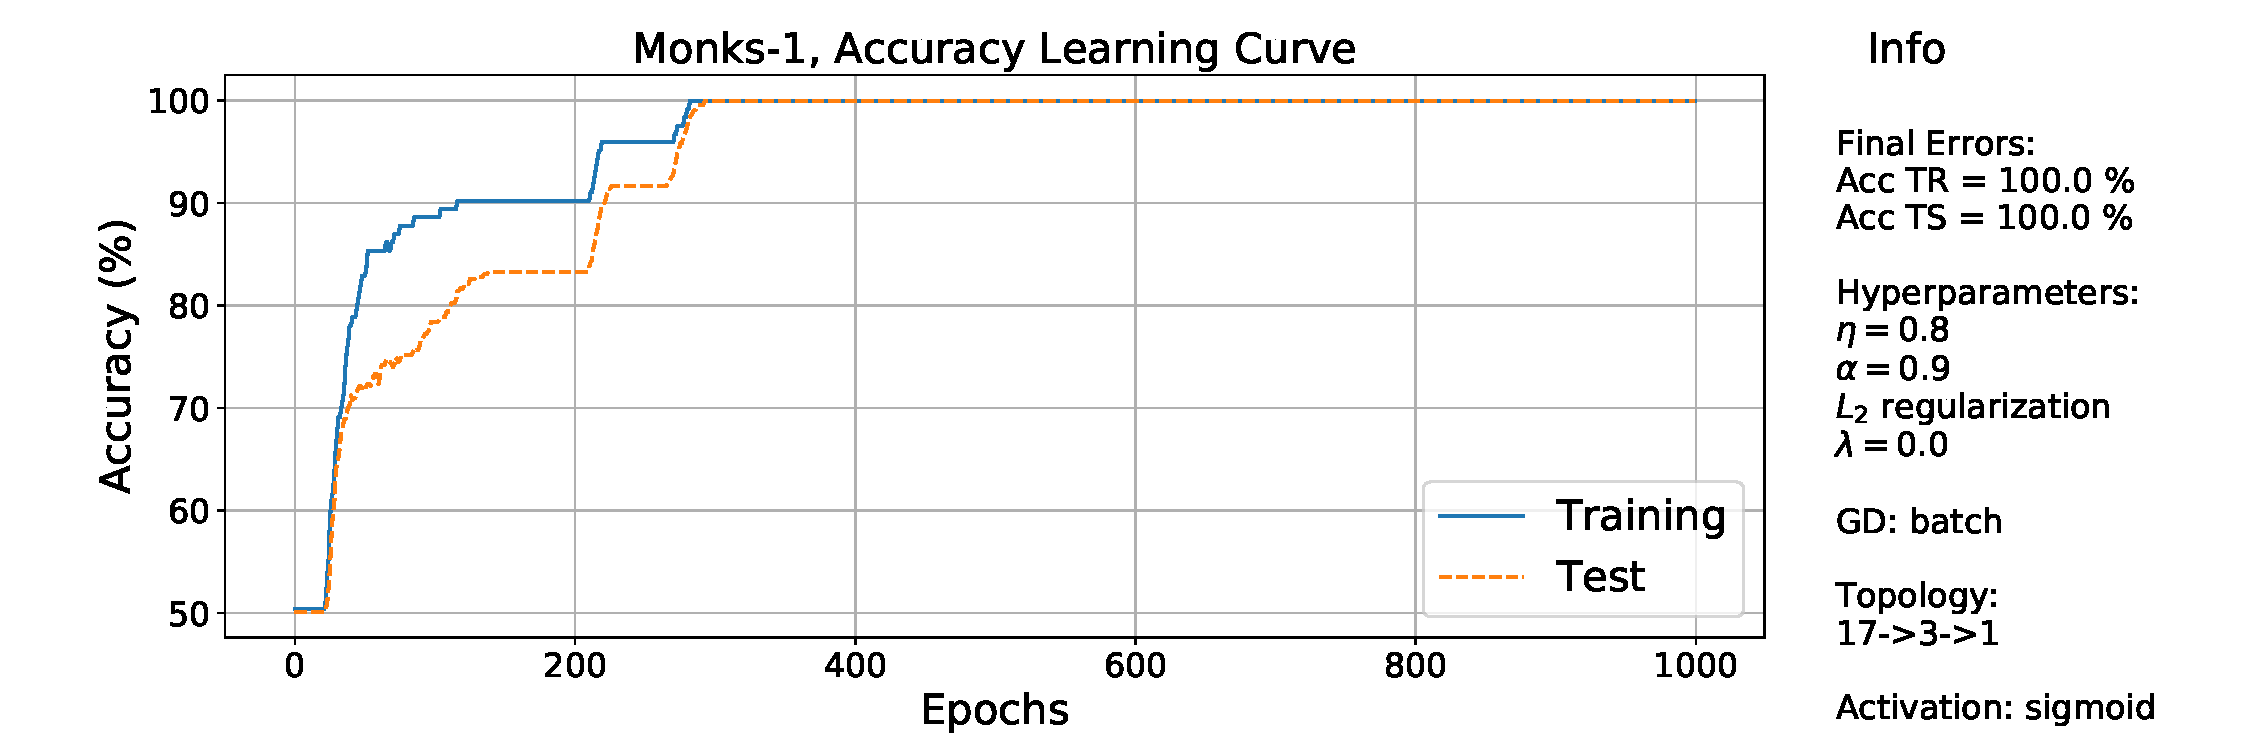
\includegraphics{img/monks_1_ACC_final_04.pdf}
            }
            \caption{}
            \label{fig:monks_1_ACC}
        \end{subfigure}
        \caption{MONKS 1 final results.}
        \label{fig:monks_1_final_results}
    \end{figure}

    \begin{figure}[htbp]
        \centering
        \begin{subfigure}{0.90\textwidth}
            \resizebox{\textwidth}{!}{
                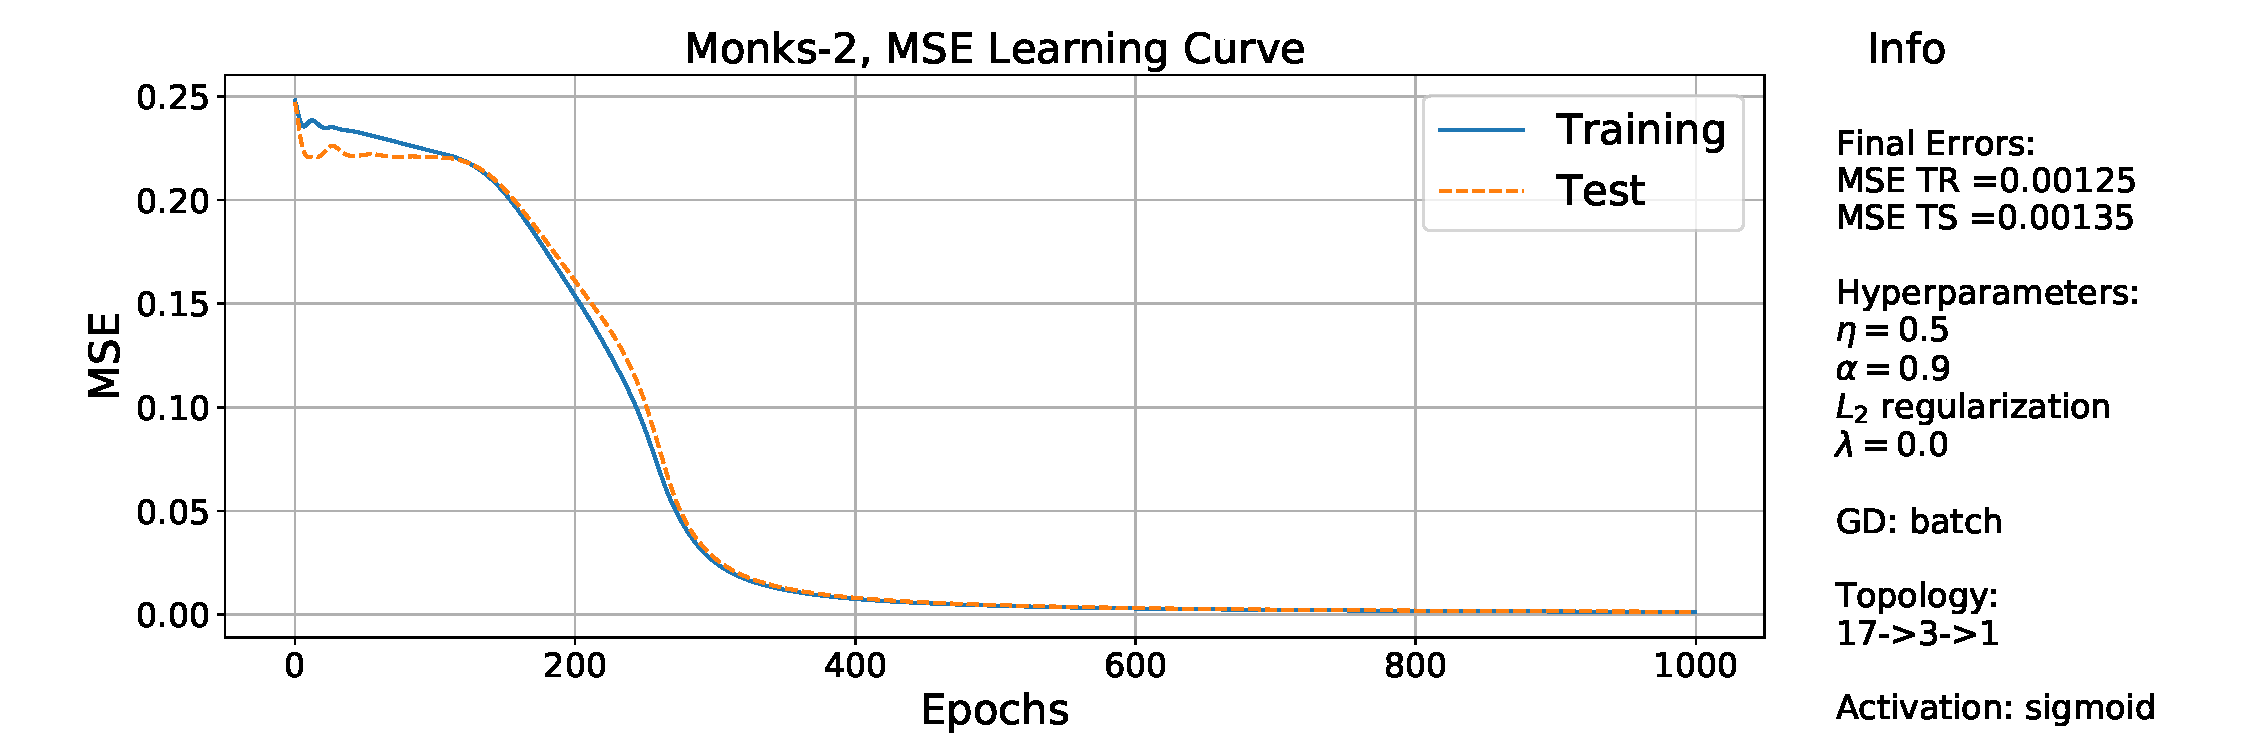
\includegraphics{img/monks_2_MSE_final_03.pdf}
            }
            \caption{}
            \label{fig:monks_2_MSE}
        \end{subfigure}
        \begin{subfigure}{0.90\textwidth}
            \resizebox{\textwidth}{!}{
                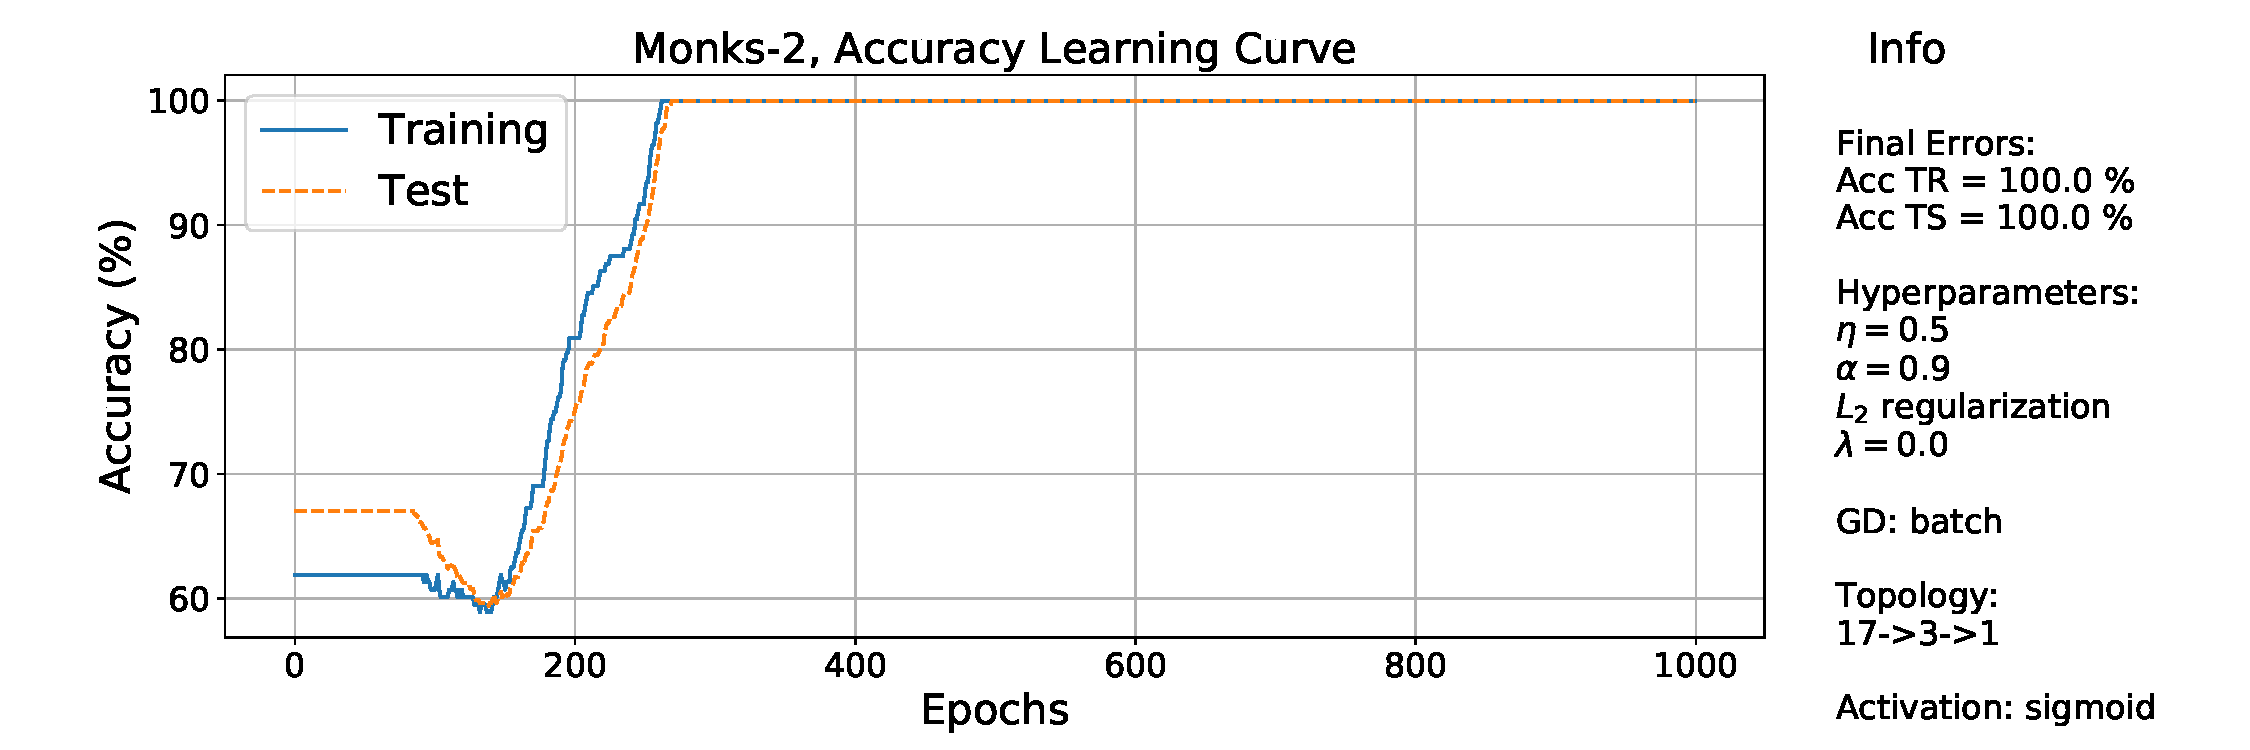
\includegraphics{img/monks_2_ACC_final_03.pdf}
            }
            \caption{}
            \label{fig:monks_2_ACC}
        \end{subfigure}
        \caption{MONKS 2 final results.}
        \label{fig:monks_2_final_results}
    \end{figure}

    \begin{figure}[htbp]
        \centering
        \begin{subfigure}{0.90\textwidth}
            \resizebox{\textwidth}{!}{
                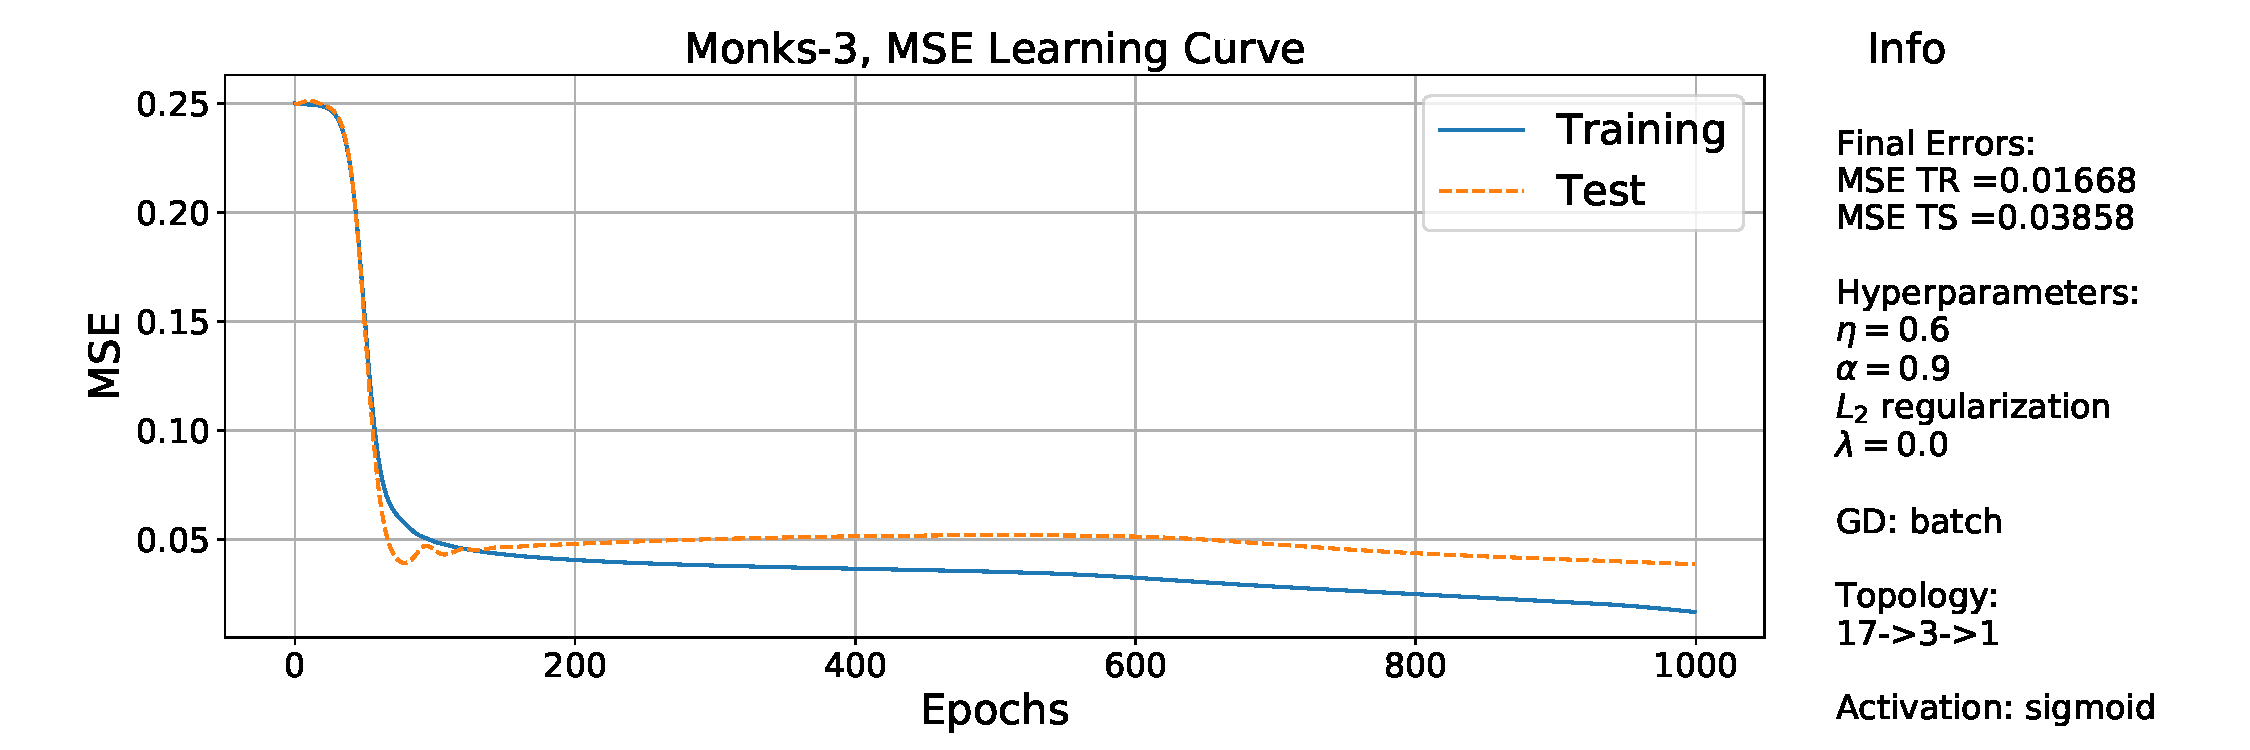
\includegraphics{img/monks_3_noreg_MSE_final_01.pdf}
            }
            \caption{}
            \label{fig:monks_3_MSE}
        \end{subfigure}
        \begin{subfigure}{0.90\textwidth}
            \resizebox{\textwidth}{!}{
                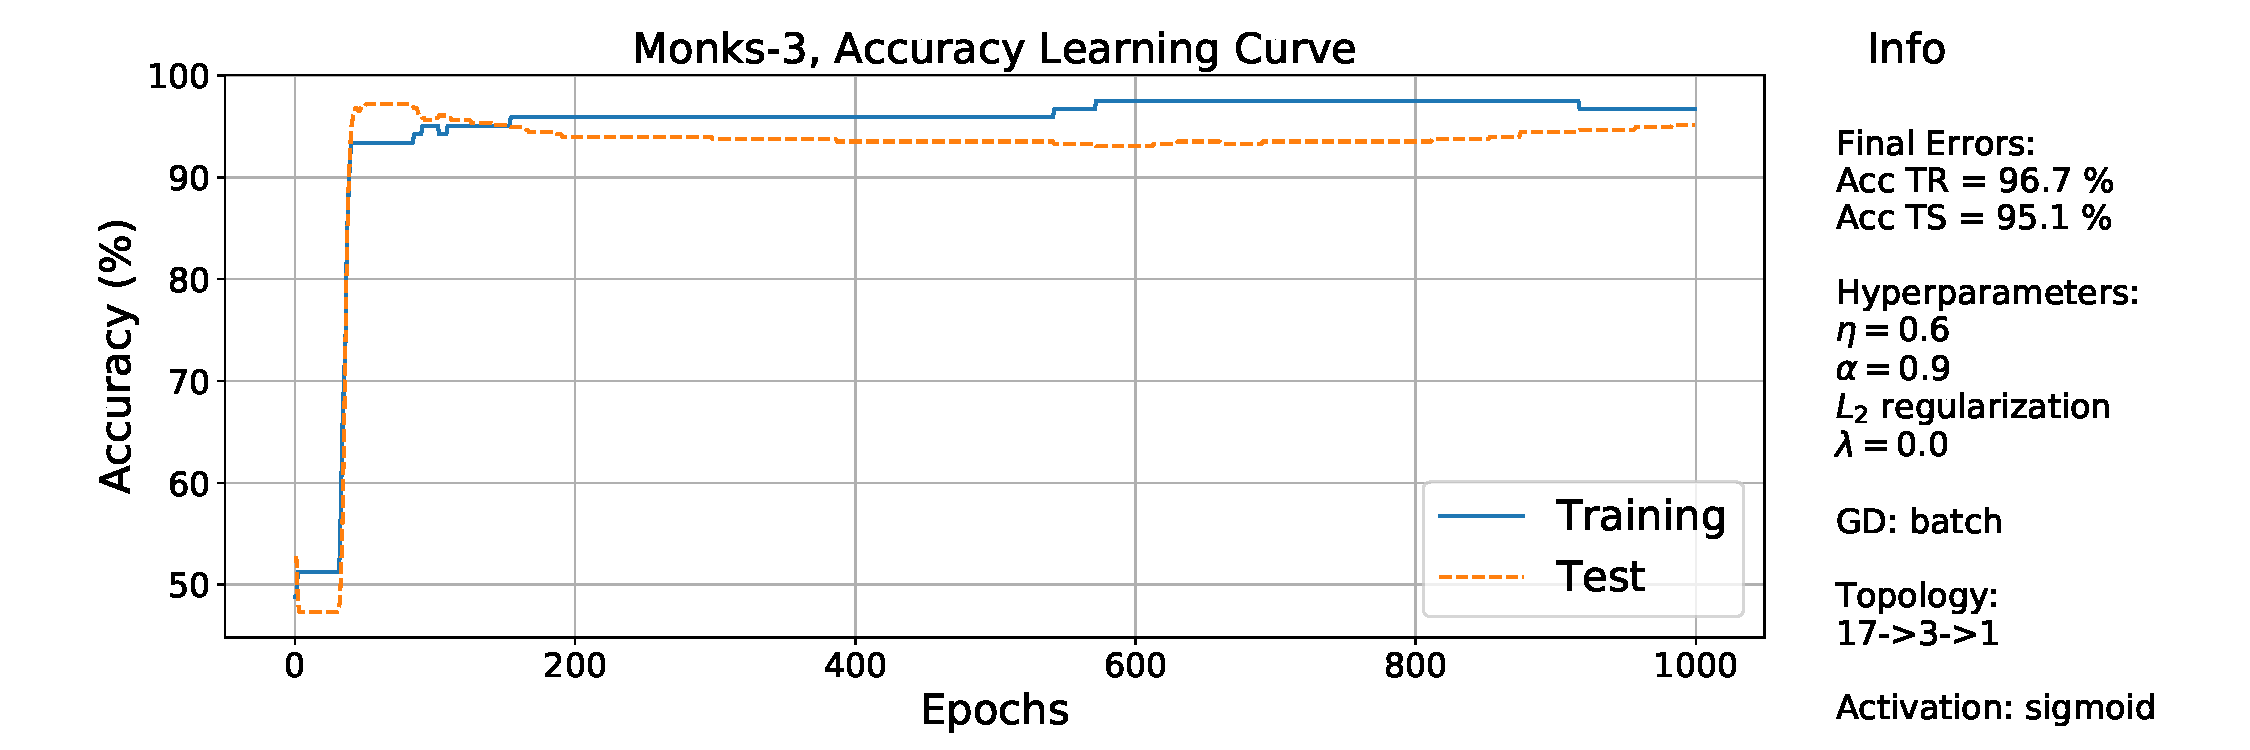
\includegraphics{img/monks_3_noreg_ACC_final_01.pdf}
            }
            \caption{}
            \label{fig:monks_3_ACC}
        \end{subfigure}
        \caption{MONKS 3 (without regularization) final results.}
        \label{fig:monks_3_final_results}
    \end{figure}

    \begin{figure}[htbp]
        \centering
        \begin{subfigure}{0.90\textwidth}
            \resizebox{\textwidth}{!}{
                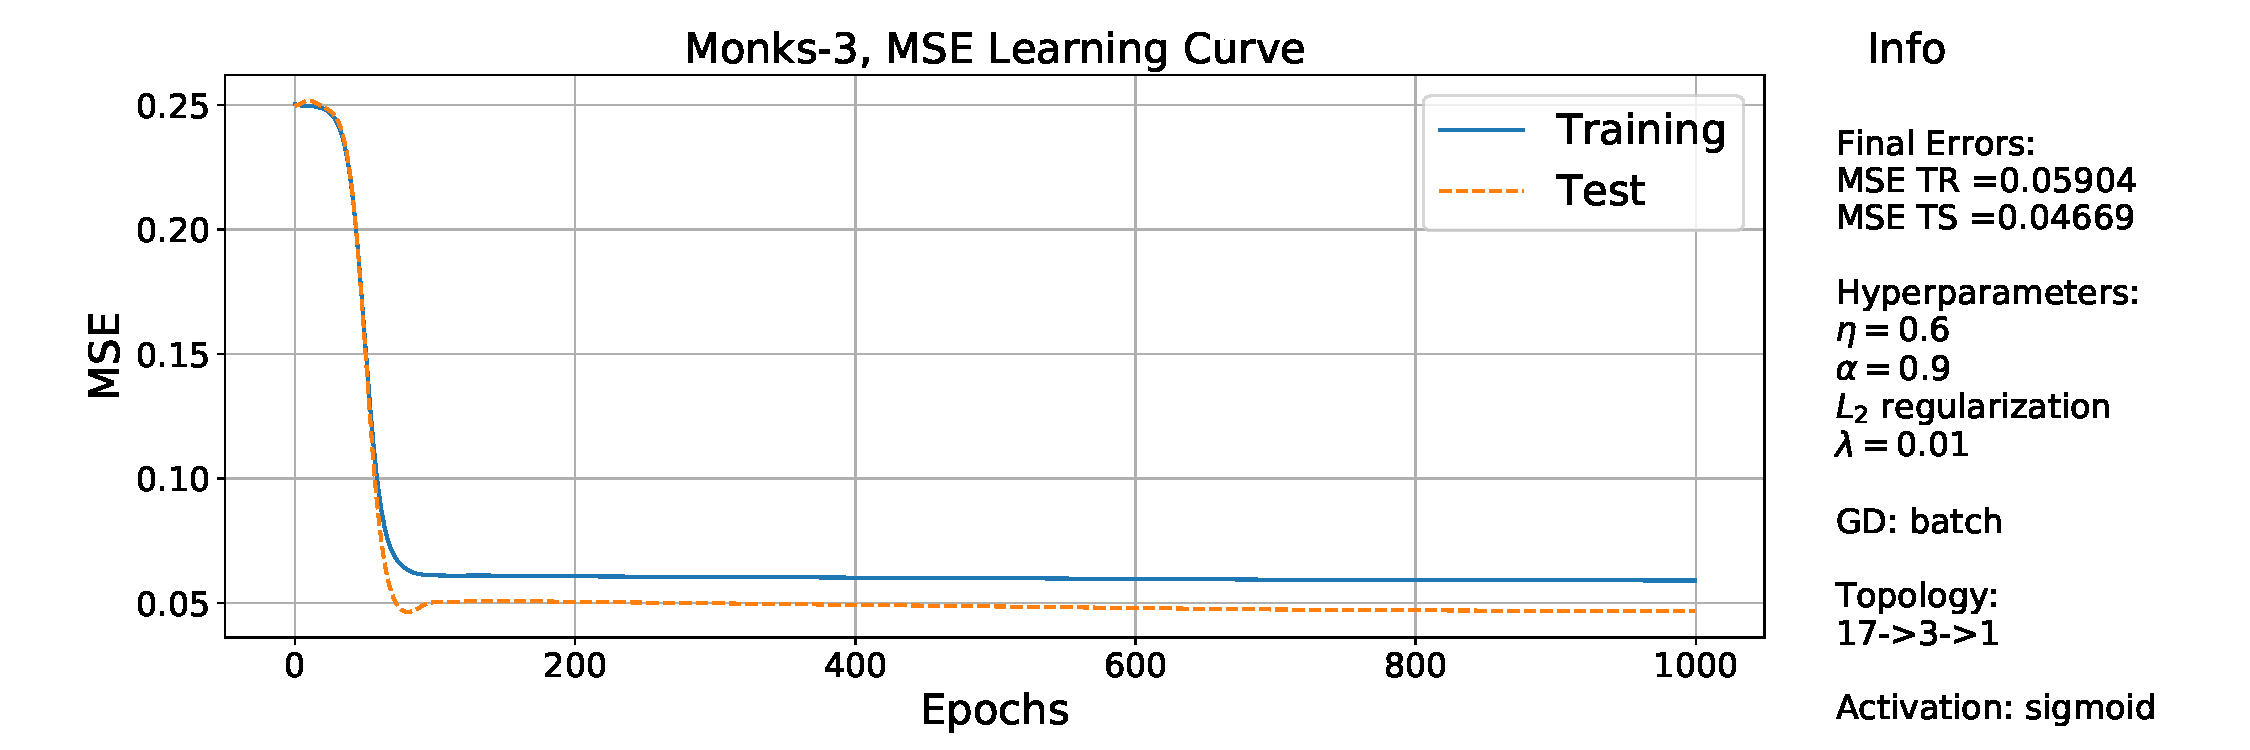
\includegraphics{img/monks_3_withreg_MSE_final_00.pdf}
            }
            \caption{}
            \label{fig:monks_3_MSE_reg}
        \end{subfigure}
        \begin{subfigure}{0.90\textwidth}
            \resizebox{\textwidth}{!}{
                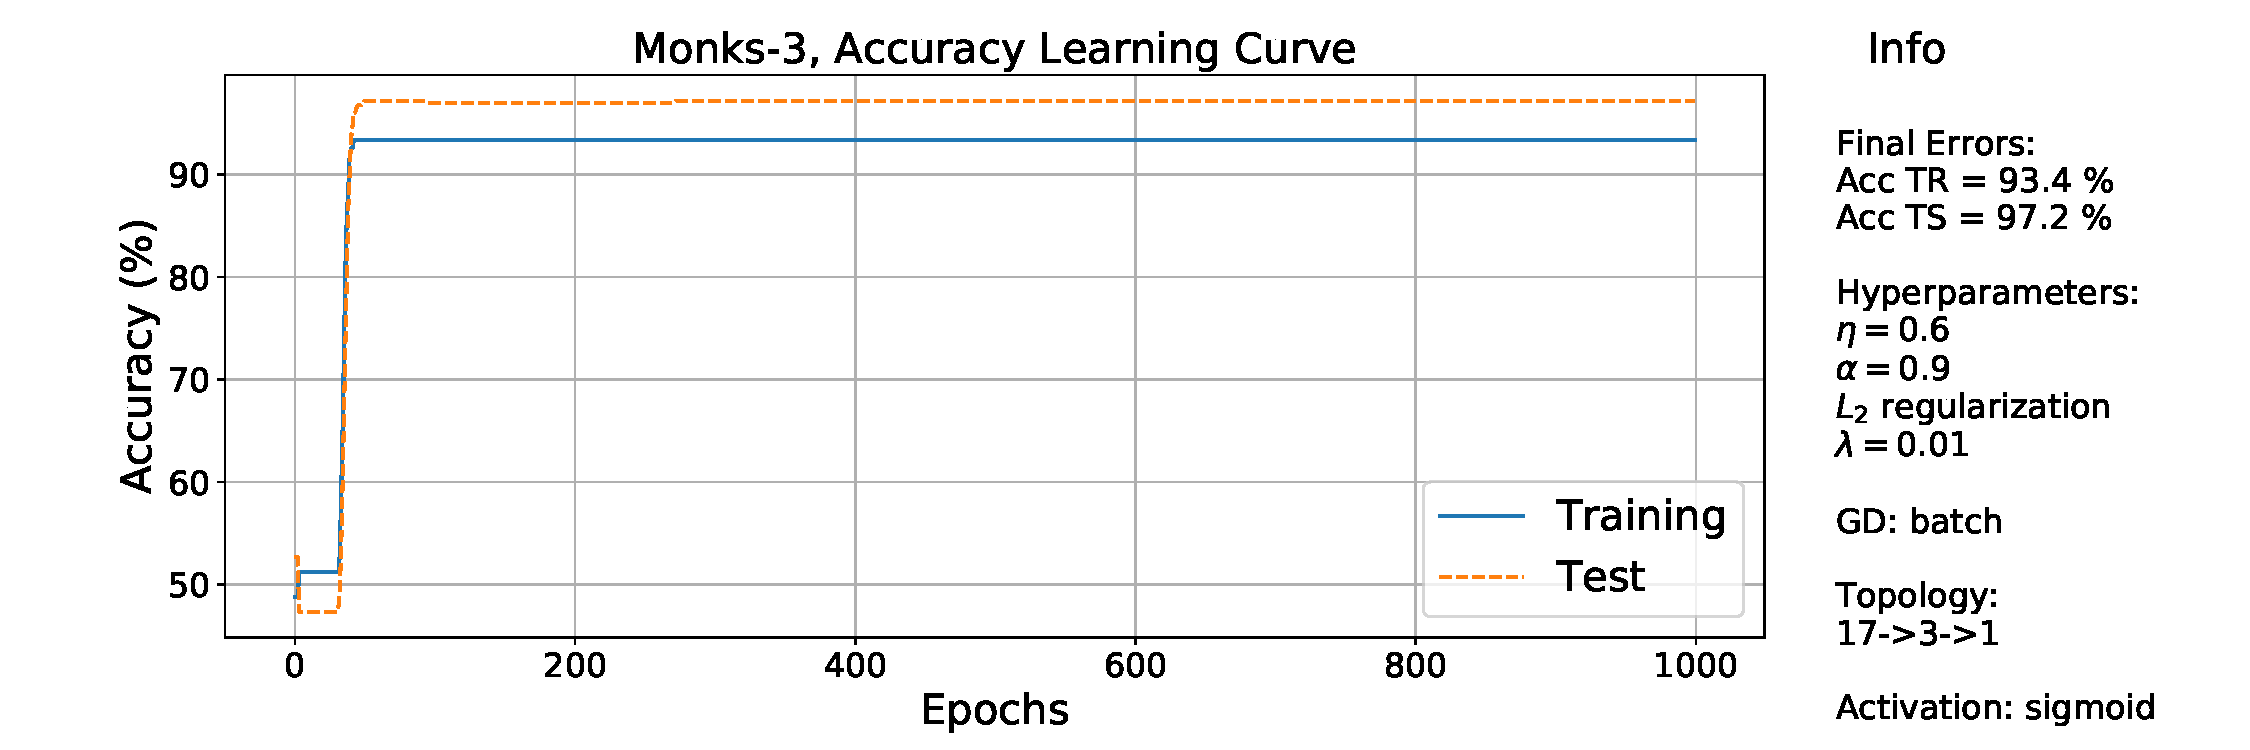
\includegraphics{img/monks_3_withreg_ACC_final_00.pdf}
            }
            \caption{}
            \label{fig:monks_3_ACC_reg}
        \end{subfigure}
        \caption{MONKS 3 (with regularization) final results.}
        \label{fig:monks_3_final_results}
    \end{figure}

    % subsection monk_s_results (end)

    \subsection{Cup results} % (fold)
    \label{sub:cup_results}
        We now proceed to detail the results we obtained for the CUP dataset. As for the MONKS dataset, we've
        employed a \textit{validation schema} consisting in an application of the \textit{random grid search}
        algorithm in conjunction with the \textit{k-fold cross validation} algorithm. As we've said before,
        we've chosen a standard value of $3$ for algorithm's $k$ parameter. In order to come up with final
        ranges for model's hyper-parameters we've performed some preliminary tests on the dataset, as for the
        MONKS dataset.

        % \begin{comment}
      %\end{comment}
        Some examples of the learning curves we discover during this preliminary phase can be seen in appendix
        \ref{sec:preliminary_trials_learning_curves_for_cup}. In table \ref{tab:hyper_ranges} you can see the
        final ranges we selected for the random grid search algorithm for the CUP dataset.

\newpage
The validation schema for the Cup dataset it is summarized by the following steps.

\begin{enumerate}
\item The original training dataset has been splitted randomly in a \textit{design set}, used for the model selection phase, and an internal \textit{test set} used only for the final models assessment.
  We have chosen a small $5\%$ sample size percentage for the test set (50 samples), because the main focus of the analysis is to perform a good model selection. %%The application of more complex validation methods such as double cross validation was beyond the available time and computing resources.
\item Preliminary 'babysitting'. The design set has been splitted into training and validation sets, with $70\%$ and $30\%$ percentages, in order to initially explore the behaviour of the neural network on the cup dataset, and to identify good parameter ranges. We tried to achieve overtraining by varying the learning rate, the number of units and momentum without using regularization approaches. We have chosen to use the \textit{relu} activation function for the hidden layer, which is faster respect to the sigmoid, and more suitable for a regression task REF?.
  We have observed that the learning time to achieve overtraining for a wide range of different number of units requires at least 2000 epochs. We fixed the maximum amount of learning time to 3000 epochs.
This learning time is quite expensive for our computing resources, so we decided to use a \textit{batch} gradient descent approach.

\item Early Stopping testing.
  The 'batch' approach allows to obtain smoother learning curves respect to minibatch/online and permits to apply easily an early stopping technique. We tested two approaches from \cite{early_stopping}.
  The $GL_{\epsilon}$ approach stops the learning process when the generalization loss exceed a defined threshold $\epsilon$, given as a percentage with respect to the minimum current value of the loss. The $PQ_{\epsilon}$ approach is similar, but take into account also the progress of the training error.
  For different hyperparameters configurations we have computed the ratio between the MEE error obtained with the two early stopping criteria and the minimum validation error of the overtrained learning curve, reported in Fig. \ref{fig:early_stop}. The early stopping methods take action only after a minimum number of epochs equal to 500, in order to avoid initial oscillation of the learning curves, and we fixed the threshold $\epsilon=1\%$. An example of early stopping computation is represented in Fig. \ref{fig:learning_early}. The results shows that the two methods are quite reliable, we opted to use the $PQ_{1\%}$ method, which in general is more robust \cite{early_stopping}.

  \begin{figure}[htbp]
    \centering
    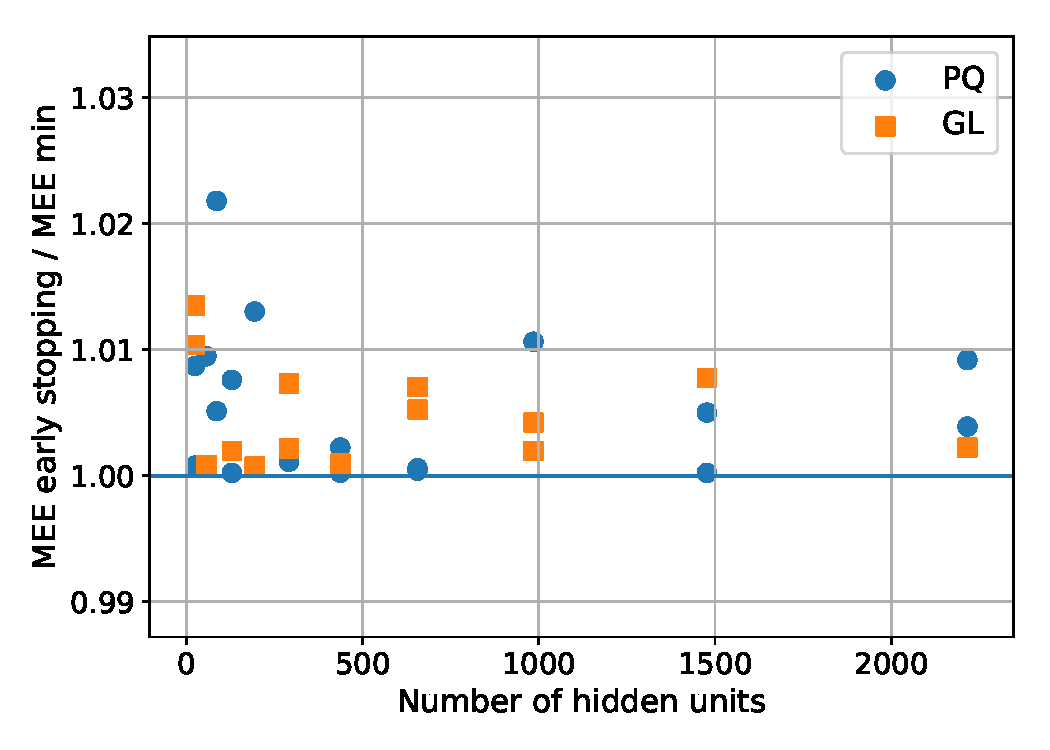
\includegraphics[width=0.90\textwidth]{img/early_stop.pdf}
    \caption{Ratio between the MEE obtained with early stopping and the minimum validation MEE.}
    \label{fig:early_stop}
  \end{figure}

    \begin{figure}[htbp]
    \centering
    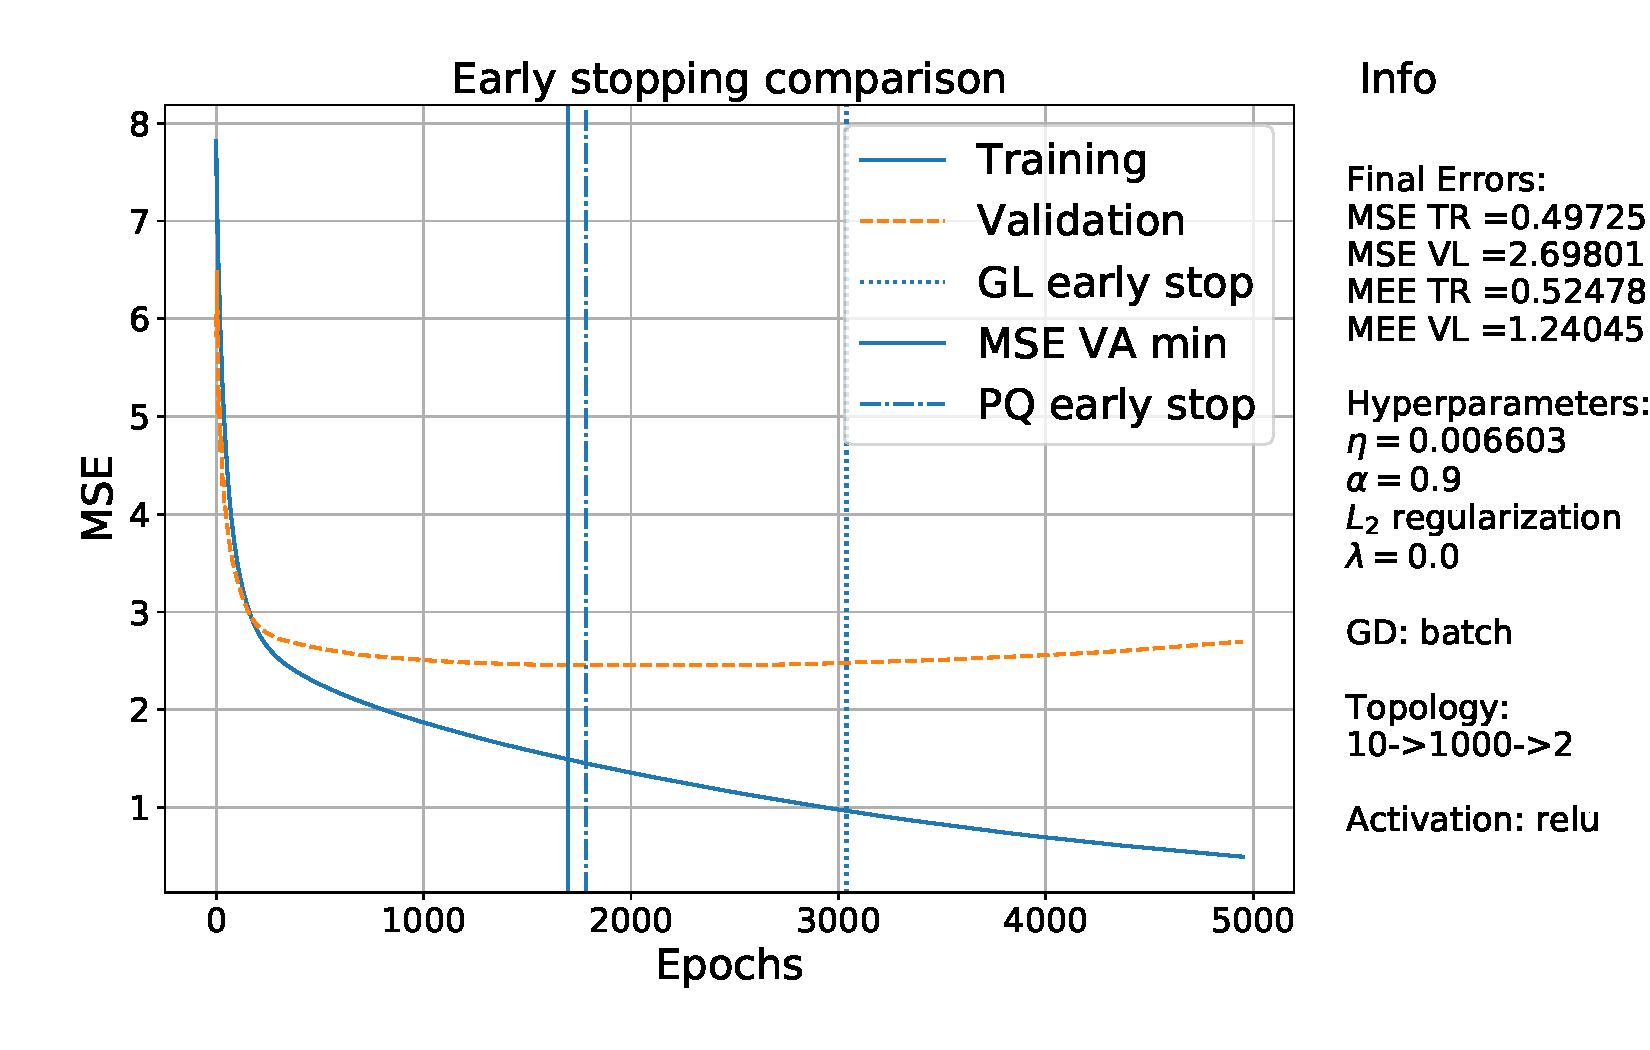
\includegraphics[width=0.90\textwidth]{img/learning_early_2.pdf}
    \caption{ Early stopping example. The vertical lines represent the early stopping points computed with $PQ_{1\%}$ and $GL_{1\%}$ methods and the point of minimum MSE on the validation curve.}

    \label{fig:learning_early}
  \end{figure}



\item Wide grid search


\item Finer grid search


\item Final model selection


\item Model assessment  
  

\end{enumerate}
        \begin{table}[hbtp]
            \centering
            \begin{tabular}{ccc }
              \toprule
                Hyper-parameter & Wide Grid & Finer Grid\\
                \midrule
                $\eta$ & $\left [ 0.08, 0.02 \right ]$ & -\\

                $\alpha$ & $0.9$ & - \\

                $\lambda$ & $0.0$ & -\\

                $\epsilon$ & $1.0\,\%$ & -\\

                hidden sizes & $\left [ 50, 2500 \right ]$ & -\\
                \midrule
            \end{tabular}
            \caption{Final hyper-parameters' ranges for the random grid search algorithm.}
            \label{tab:hyper_ranges}
          \end{table}







    % subsection cup_results (end)

% section experiments (end)

%------------------------------------------------
\clearpage

\section{Conclusions} % (fold)
\label{sec:conclusions}

% section conclusions (end)

%----------------------------------------------------------------------------------------
%   REFERENCE LIST
%----------------------------------------------------------------------------------------

\begin{thebibliography}{99} % Bibliography - this is intentionally simple in this template
    \bibitem{deep_learning}
    Ian Goodfellow, Yoshua Bengio and Aaron Courville.
    \textit{Deep Learning}, MIT Press, 2016.

    \bibitem{random_search}
    James Bergstra and Yoshua Bengio.
    \textit{Random Search for Hyper-parameter Optimization}, J. Mach. Learn. Res. 13, pp. 281-305, 2012.

    \bibitem{early_stopping}
    Prechelt Lutz.
    \textit{Early Stopping - But When?}, Montavon G., Orr G.B., Müller KR. (eds) Neural Networks: Tricks of the
    Trade. Lecture Notes in Computer Science, vol 7700. Springer, Berlin, Heidelberg, 2012.

    \bibitem{initialization}
    Xavier Glorot and Yoshua Bengio.
    \textit{Understanding the difficulty of training deep feedforward neural networks},
    Proceedings of the Thirteenth International Conference on Artificial Intelligence and Statistics, pp.
    249-256, 2010.
\end{thebibliography}

\newpage

%----------------------------------------------------------------------------------------

%----------------------------------------------------------------------------------------
%   APPENDIX
%----------------------------------------------------------------------------------------

\pagenumbering{roman}
\begin{appendices}
    \section{Preliminary trials' learning curves for MONKS} % (fold)
    \label{sec:preliminary_trials_learning_curves}
    % section preliminary_trials_learning_curves (end)

    \section{Preliminary trials' learning curves for CUP} % (fold)
    \label{sec:preliminary_trials_learning_curves_for_cup}

    % section preliminary_trials_learning_curves_for_cup (end)

    \section{How to run the code} % (fold)
    \label{sec:how_to_run_the_code}
        In this section we show how to run our code.
    % section how_to_run_the_code (end)

\end{appendices}

%----------------------------------------------------------------------------------------

\end{document}
